%%%%%%%%%%%%%%%%%%%%%%%%%%%%%%%%%%%%%%%%%%%%%%%%%%%%%%%%%%%%%%%%%%%%%%%%%%%%%%%%%%
\begin{frame}[fragile]\frametitle{}
\begin{center}
{\Large Functions}
\end{center}
\end{frame}

%%%%%%%%%%%%%%%%%%%%%%%%%%%%%%%%%%%%%%%%%%%%%%%%%%%%%%%%%%%
 \begin{frame}[fragile]\frametitle{Functions}
\begin{itemize}
\item Takes many inputs and produces one output
\item $f(x) = x + 2$
\item $f(3)=?$
\item This function is a line, with $y$ is same as $f(x)$
\end{itemize}
\begin{center}
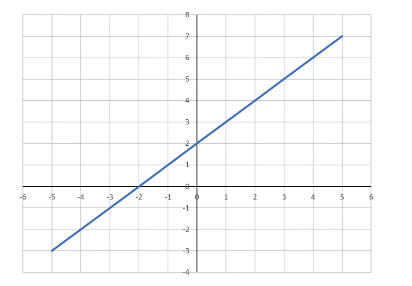
\includegraphics[width=0.5\linewidth,keepaspectratio]{func1}
\end{center}
\end{frame}

%%%%%%%%%%%%%%%%%%%%%%%%%%%%%%%%%%%%%%%%%%%%%%%%%%%%%%%%%%%
 \begin{frame}[fragile]\frametitle{Functions}
\begin{itemize}
\item Another example : $g(x) = 10/x$
\item $g(5)=?$
\item $g(0)=undefined$
\item Set of numbers for which the function is defined is called ``Domain''.
\item For $g$ domain is $\{x \in \mathbb{R} | x \neq 0\}$
\end{itemize}
\begin{center}
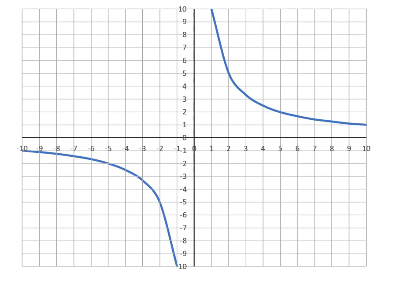
\includegraphics[width=0.5\linewidth,keepaspectratio]{func2}
\end{center}
\end{frame}

%%%%%%%%%%%%%%%%%%%%%%%%%%%%%%%%%%%%%%%%%%%%%%%%%%%%%%%%%%%
 \begin{frame}[fragile]\frametitle{Exercise}
$h(x) = 2 \sqrt{x}, x \geq 0$

\begin{lstlisting}
def h(x):
    if x >= 0:
        import numpy as np
        return 2 * np.sqrt(x)

import numpy as np
from matplotlib import pyplot as plt

x = range(-100, 101)
y = [h(a) for a in x]

plt.xlabel('x')
plt.ylabel('h(x)')
plt.grid()

plt.plot(x,y, color='purple')
plt.plot(0,h(0.0000001), color='purple', marker='o', markerfacecolor='w', markersize=8)
plt.show()
\end{lstlisting}
\end{frame}

%%%%%%%%%%%%%%%%%%%%%%%%%%%%%%%%%%%%%%%%%%%%%%%%%%%%%%%%%%%
 \begin{frame}[fragile]\frametitle{Plot}
\begin{center}
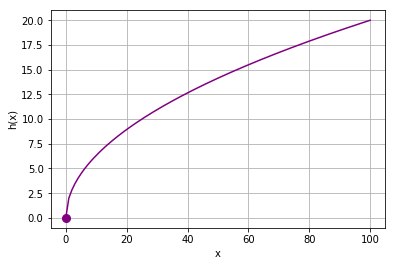
\includegraphics[width=0.5\linewidth,keepaspectratio]{func3}
\end{center}
\end{frame}


%%%%%%%%%%%%%%%%%%%%%%%%%%%%%%%%%%%%%%%%%%%%%%%%%%%%%%%%%%%
 \begin{frame}[fragile]\frametitle{Computable Functions}
\begin{itemize}
\item $p(x) = x^2 - 5x + 6$
\item Computers can easily compute, once $x$ is given, as it involves just multiplications and additions.
\item Is it easy to compute Trigonometric functions? like $\sin,\cos$.
\item Right angle triangle definition
\begin{center}
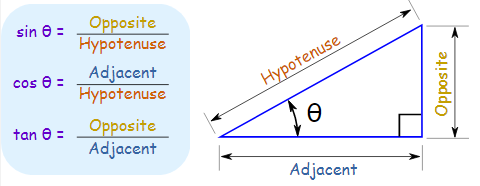
\includegraphics[width=0.5\linewidth,keepaspectratio]{trig}
\end{center}
\item Is it a complete definition? Can it handle $\theta > 90$?
\end{itemize}
\end{frame}

%%%%%%%%%%%%%%%%%%%%%%%%%%%%%%%%%%%%%%%%%%%%%%%%%%%%%%%%%%%
 \begin{frame}[fragile]\frametitle{Functions}
\begin{itemize}
\item To go beyond $90$ we may use addition formula $\sin(a+b) = \sin a \cos b + \cos a \sin b$
\item But still, we need formulation thats more encompassing. Thats given by circle.
\item A real-line is divided into parts of $2\pi$. One of the parts, say $0-2\pi$ is wrapped around a circle with unit radius.
\item Any real number will have a place on the circumference.
\item This point's x coordinate gives $\cos number$, y coordinate gives $\sin number$.
\begin{center}
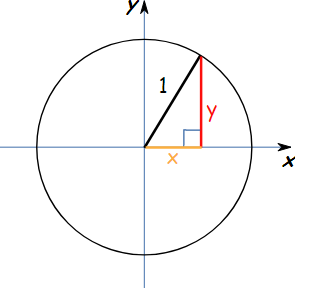
\includegraphics[width=0.3\linewidth,keepaspectratio]{circ}
\end{center}
\end{itemize}
\end{frame}


%%%%%%%%%%%%%%%%%%%%%%%%%%%%%%%%%%%%%%%%%%%%%%%%%%%%%%%%%%%
 \begin{frame}[fragile]\frametitle{Functions: Series expansion}
\begin{itemize}
\item For computers to compute, you need expression in terms of multiplication and additions.
\item Functions like Trigonometric (Transcendental) are not like that.
\item Taylor's series (aka Mcluaren) given generic way of expressing functions as series
\item $f(x=0) = \sum_{n=0}{\infty} \frac{f^n(0)}{n!} x^n$
\item $\sin x = x - \frac{x^3}{3!} + \frac{x^5}{5!} + \ldots$
\end{itemize}
\end{frame}

%%%%%%%%%%%%%%%%%%%%%%%%%%%%%%%%%%%%%%%%%%%%%%%%%%%%%%%%%%%
\begin{frame}[fragile]\frametitle{}
\textbf{Definition}
A \underline{function of two variables} is a rule which assigns to each pair $(x,y)$ of real numbers in a set $D$ called the \underline{domain} a unique real value denoted by $f(x,y)$.  \\ 
The set of all values attained by $f$ is the \underline{range} of $f$.
 

\textbf{Example}
The area of a rectangle is a function of its length $\ell$ and its width $w$.  So, it can be thought of as a function of two variables $A(\ell,w)=\ell w$.
 

\textbf{Convention}  
If an explicit rule is given for a function of two or more variables and the domain is not specified, then the domain is understood to be the set of all possible inputs for which the explicit rule gives a well defined real number.

\end{frame}



%%%%%%%%%%%%%%%%%%%%%%%%%%%%%%%%%%%%%%%%%%%%%%%%%%%%%%%%%%%
\begin{frame}[fragile]\frametitle{}

\textbf{Example}
What is the domain of the function $f(x,y)=\ln(x^2-y^2)$?
  

\textbf{Note}
If a function arises in an application then the domain maybe determined by the application itself.
  

\textbf{Example}
Suppose that $V(r,h)=\pi r^2h$ is the volume of a cylindrical water tank with radius $r$ and height $h$.  What is the domain of $V$.


\textbf{Example}
Find the domain and range of the function $f(x,y)= \sqrt{16-x^2-y^2}$.


\end{frame}

%%%%%%%%%%%%%%%%%%%%%%%%%%%%%%%%%%%%%%%%%%%%%%%%%%%%%%%%%%%
\begin{frame}[fragile]\frametitle{}

\textbf{Definition}
Suppose that $f(x,y)$ is a function with domain $D$.  The \underline{graph} of $f$ is the set $\{(x,y,f(x,y)) \ |\ (x,y)\in D\}$.
 

\textbf{Example}
Draw the graph of the function $h(x,y)= 2x^2 + y^2$.

\end{frame}

%%%%%%%%%%%%%%%%%%%%%%%%%%%%%%%%%%%%%%%%%%%%%%%%%%%%%%%%%%%
\begin{frame}[fragile]\frametitle{}
\textbf{Definition}
The \underline{level curves} of a function $f(x,y)$ are the curves in $\mathbb R^3$ with equations $f(x,y)=k$ where $k\in \mathbb R$ is a constant.
 

\textbf{Note}
The level curves of $f(x,y)$ are the traces of the graph of $f(x,y)$ in the plane $z=k$.
 

\textbf{Example}
Compute the level curves of $f(x,y)=\sqrt{16-x^2-y^2}$.

\end{frame}

%%%%%%%%%%%%%%%%%%%%%%%%%%%%%%%%%%%%%%%%%%%%%%%%%%%%%%%%%%%
\begin{frame}[fragile]\frametitle{}
 
\textbf{Definition}
 A \underline{function of $n$ variables} is a rule that assigns to each $n$-tuple $(x_1,\dots, x_n)$ in some subset $D$ or $\mathbb R^n$ a real number $f(x_1,x_2,\dots,x_n)$. \\   
 The set $D$ is the \underline{domain} of $f$.



\textbf{Note}
\begin{enumerate}
 \item  The graph of a function of $n$ variables naturally lives in $\mathbb R^{n+1}$ which is not easily represented when $n>2$.  
 \item  When $n=3$, we can gain some insight by considering the level surfaces $f(x,y,z)=k$, where $k\in \mathbb R$ is constant.  
 \item  When a function of $n$ variables is given by a rule and the domain is not specified we follow the same convention as in the $n=2$ case.  That is, we take the domain to be the set of all values $\vec{x}\in\mathbb R^n$ for which the rule for $f(\vec{x})$ gives a well-defined real number.
\end{enumerate}

\end{frame}


%%%%%%%%%%%%%%%%%%%%%%%%%%%%%%%%%%%%%%%%%%%%%%%%%%%%%%%%%%%
\begin{frame}[fragile]\frametitle{}
 
\textbf{Example}
 Find the domain and range of the function $f(x,y,z)= \ln(16-x^2-y^2-z^2)$.  Plot some of its level surfaces.

\end{frame}

